\documentclass[14pt, aspectratio=169, handout]{beamer}
\usetheme{Copenhagen}
\usecolortheme{seahorse}
\setbeamertemplate{navigation symbols}{}
\setbeamertemplate{headline}{}

%\usepackage{pgfpages}
%\pgfpagesuselayout{4 on 1}[a4paper, border shrink=5mm]

\usepackage{graphicx} % Required for inserting images
\usepackage{multicol}
%\usepackage{enumitem}
\usepackage{amsfonts}
\usepackage{amsmath}
\usepackage{xcolor}

\definecolor{darkblue}{RGB}{0, 0, 139}
\definecolor{lightblue}{RGB}{173, 216, 230}

\title{SST1 Übungsstunde 4}
\author{Matteo Dietz}
\date{October 2025}

\begin{document}

\maketitle

\begin{frame}{Themenüberblick}
    \begin{itemize}
        \item \textbf{Repetition: Zeitinvarianz}
        \item[] 
        \item \textbf{Analoge LTI Systeme im Zeitbereich}:
        \item[] Impulsantwort
        \item[] Faltung, Eigenschaften der Faltung, Graphische Faltung
        \item[] Eigenschaften der Impulsantwort
    \end{itemize}
\end{frame}

\begin{frame}{Aufgaben für diese Woche}
    \begin{itemize}
        \item[] \underline{\textbf{31}}, \underline{\textbf{33}}, 34, \underline{\textbf{35}}, 36, \underline{\textbf{37}}, \underline{\textbf{38}}, \underline{\textbf{39}}, \underline{\textbf{40}}, \underline{\textbf{41}}, \underline{\textbf{42}}, \underline{\textbf{43}}, 44, \underline{\textbf{45}}
        \item[] 
        \item[] Die \underline{\textbf{fettgedruckten}} Übungen empfehle ich, weil sie wesentlich zu eurem Verständnis der Theorie beitragen und/oder sehr prüfungsrelevant sind.
    \end{itemize}
\end{frame}

\begin{frame}{Repetition: Zeitinvarianz}
    $$Hx(t) = t \cdot x(t) \hspace{3cm} T_\tau x(t) = x(t-\tau)$$
    \vspace*{-0.75cm}
    \begin{center}
        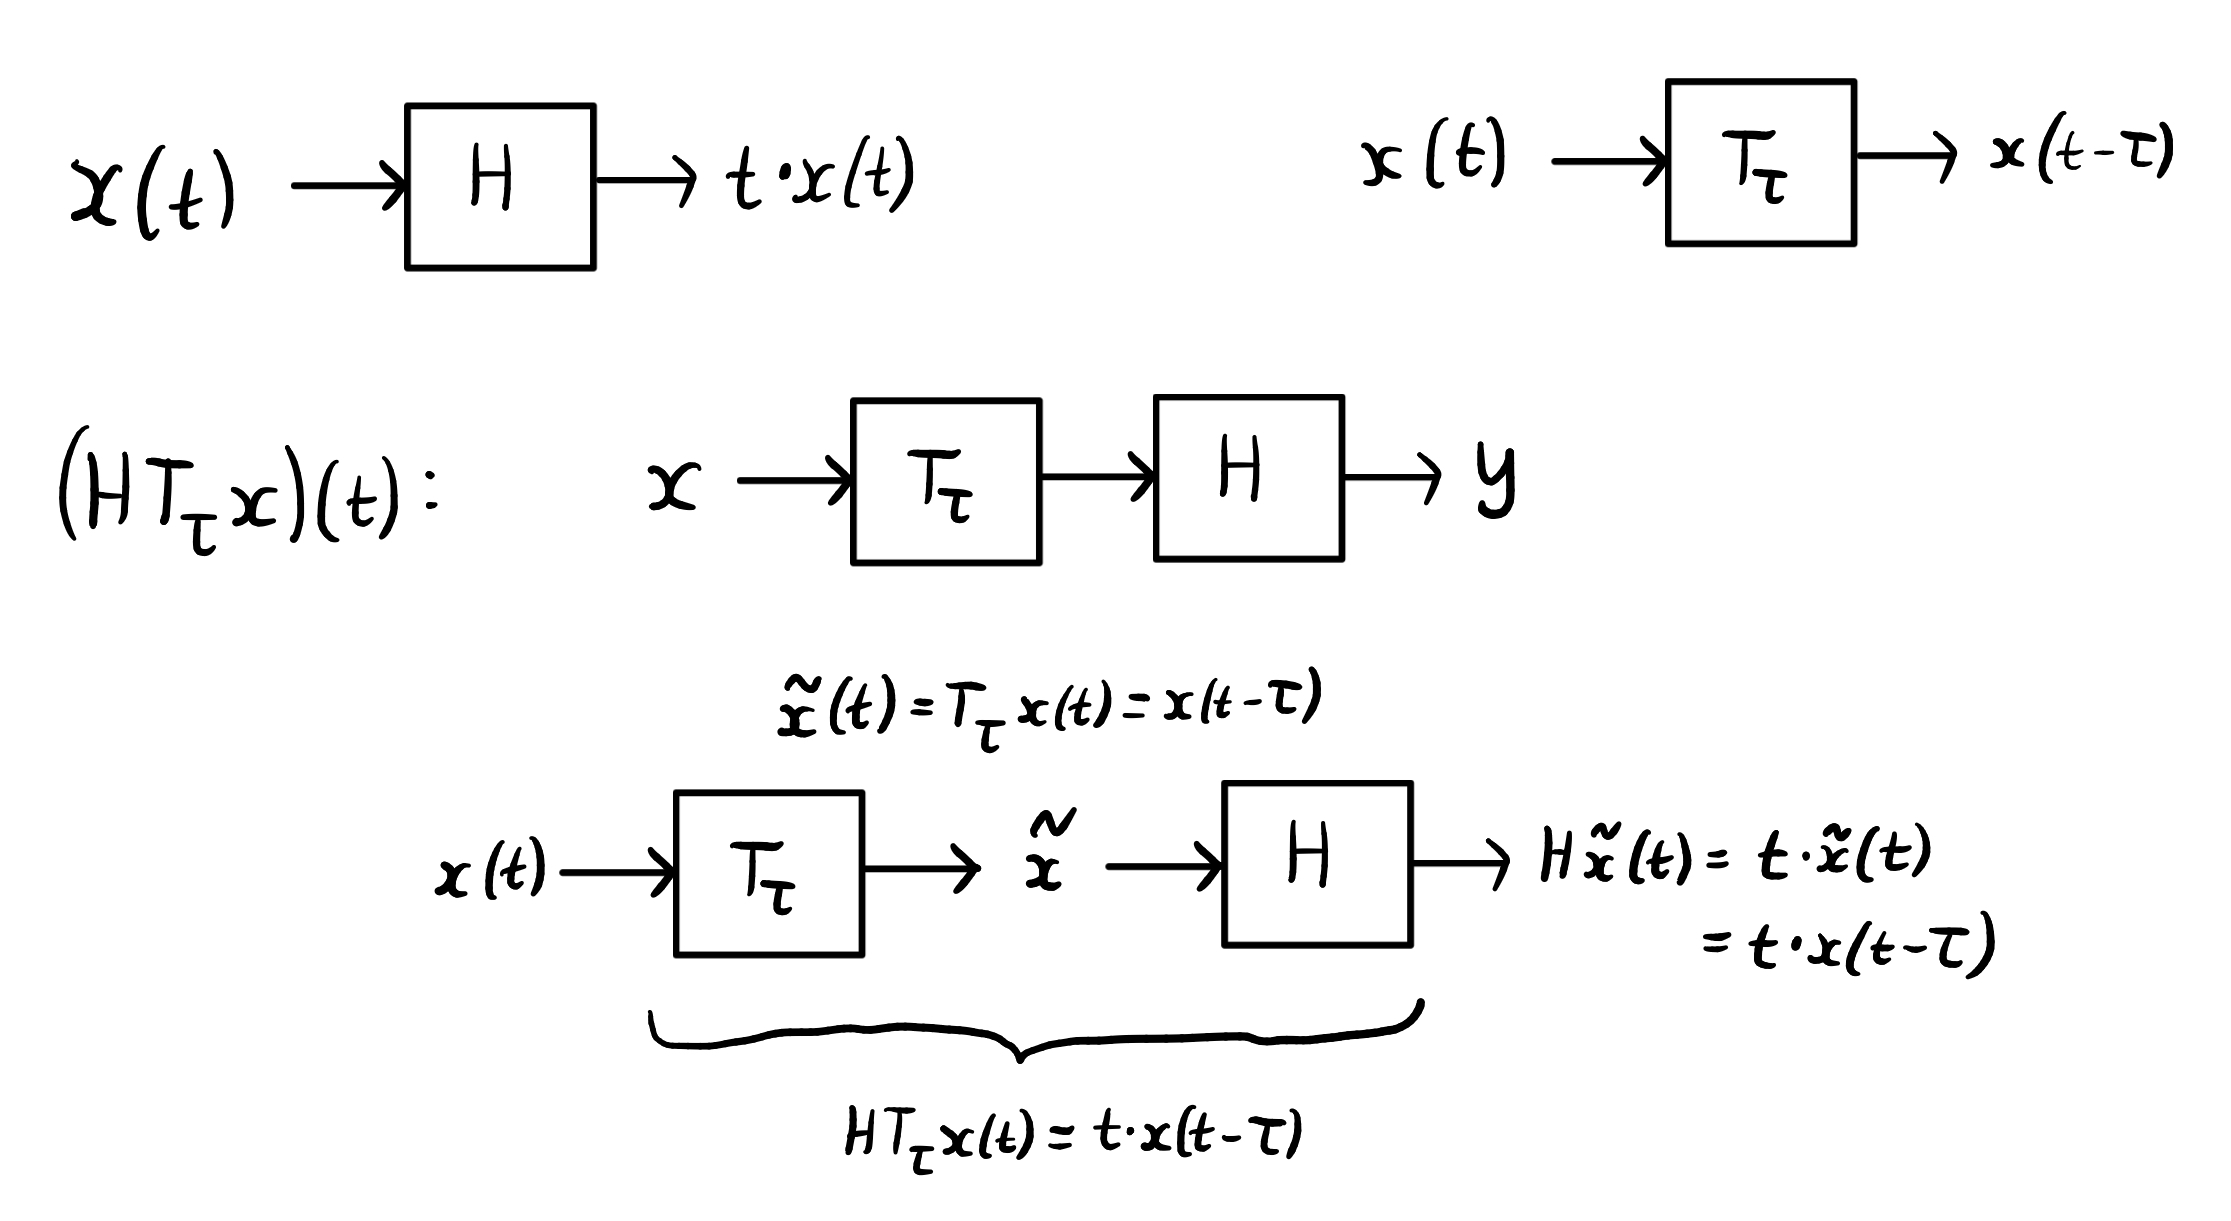
\includegraphics[width=0.8\linewidth]{figures/Zeitverschiebung.jpg}
    \end{center}
\end{frame}

\begin{frame}{Beispiel}
    \vspace*{-0.32cm}
    \begin{center}
        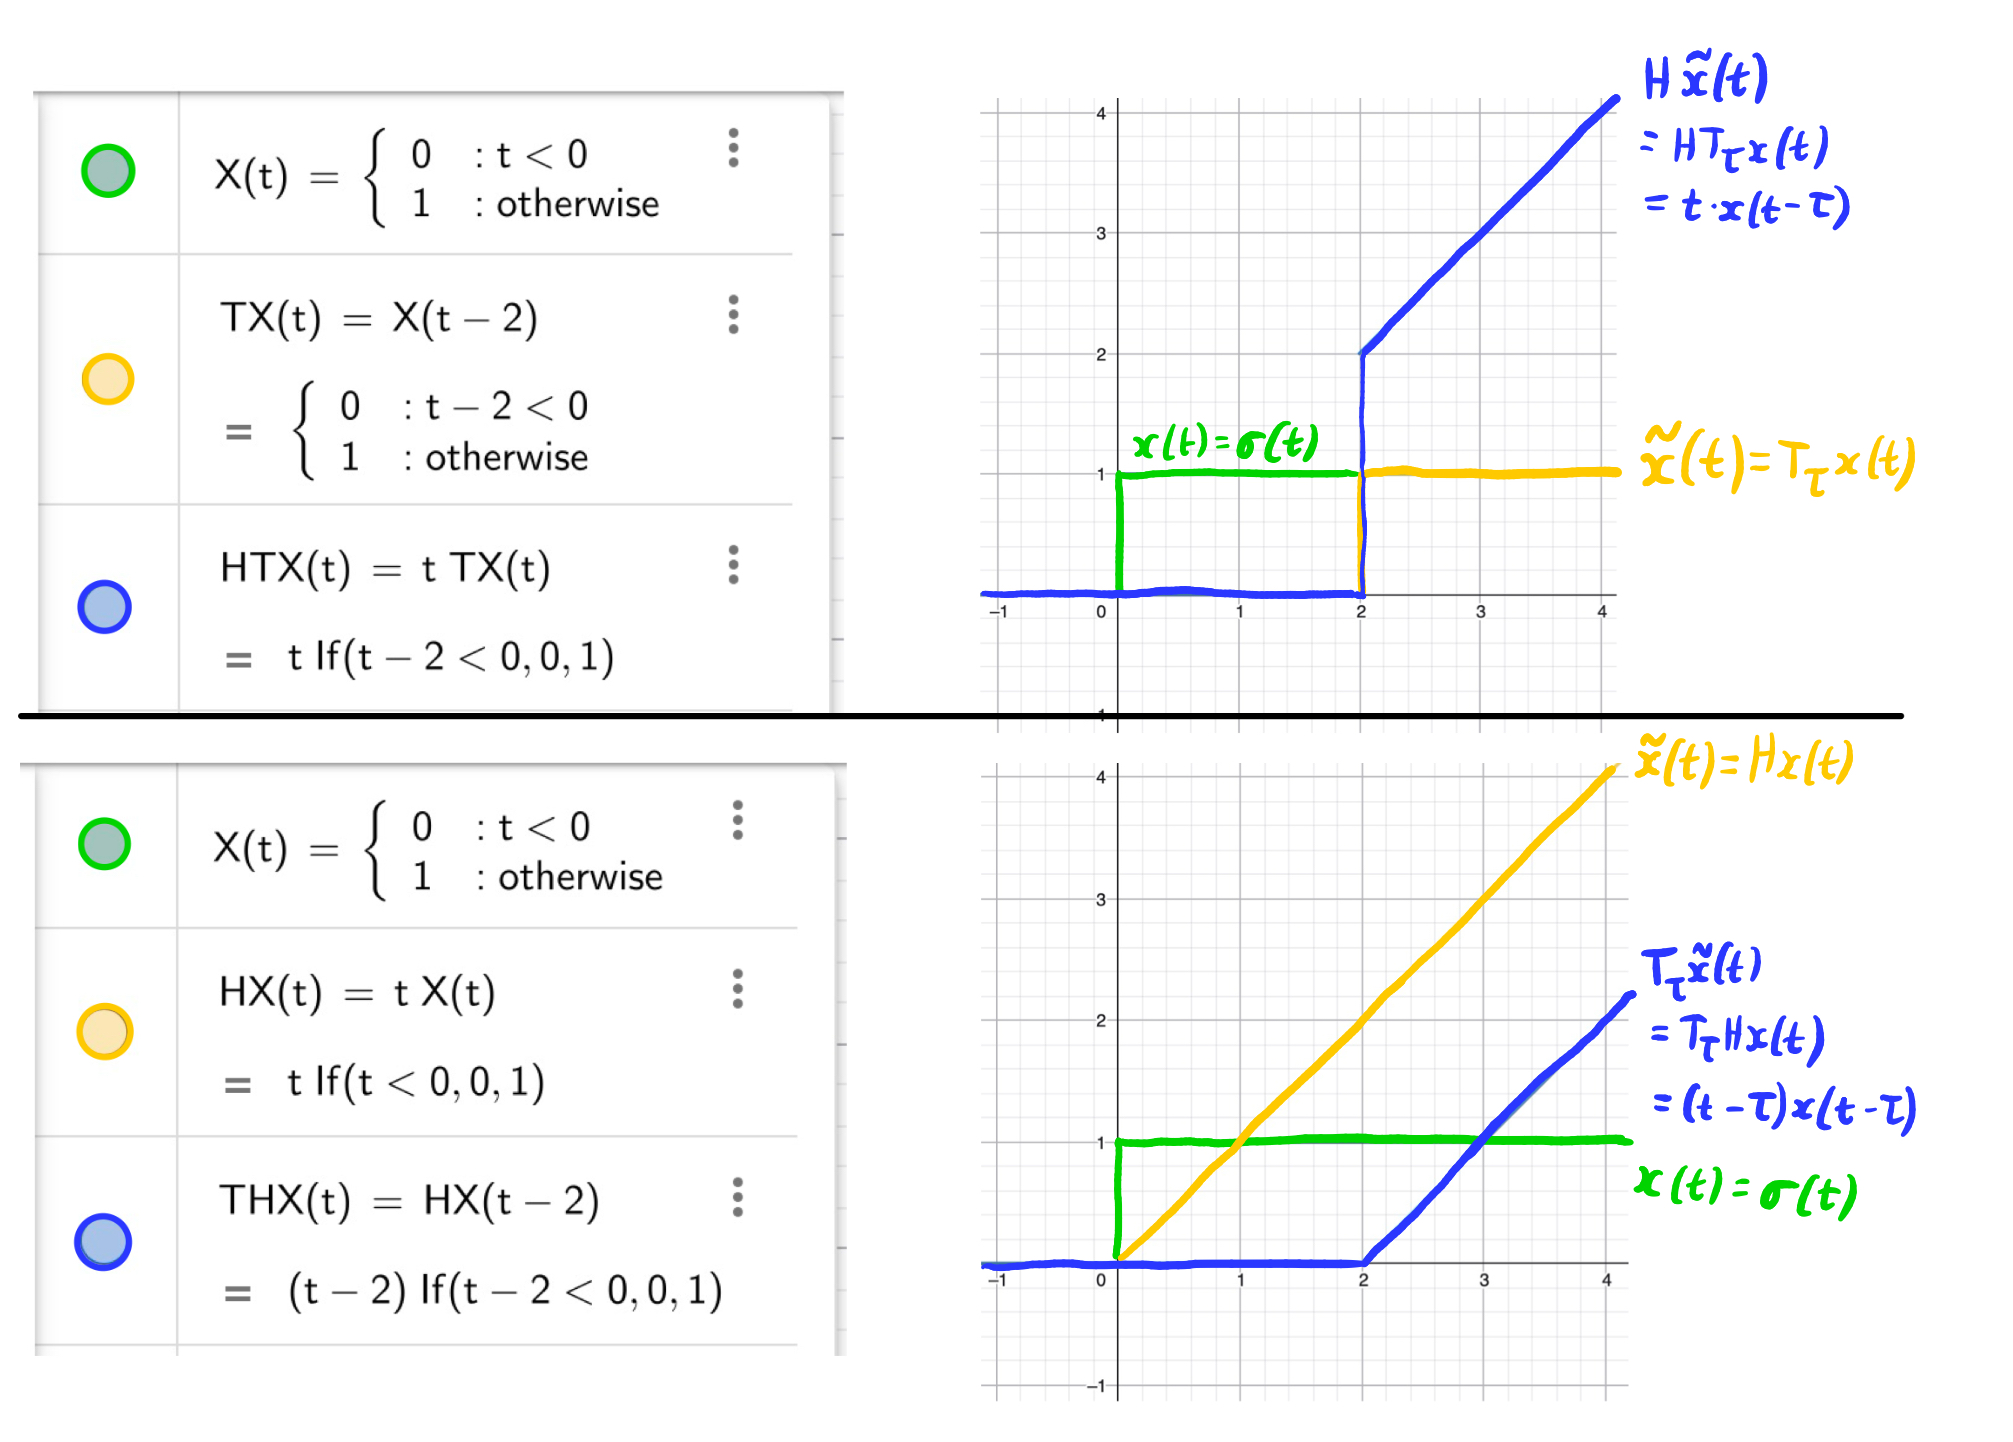
\includegraphics[width=0.8\linewidth]{figures/Zeitverschiebung_bsp.jpg}
    \end{center}
\end{frame}

\begin{frame}{Punktenotation (aus Lösung 30.c) \& 28)}
    \begin{itemize}
        \item $(Hx(\cdot -\tau))$ bedeutet: $H$ wirkt auf das verschobene Signal $x(t-\tau) = (T_\tau x)(t)$, also:
        $$(Hx(\cdot -\tau))(t) = (HT_\tau x)(t) \textcolor{blue}{\; = tx(t-\tau)}$$
        \item[]
        \item $(Hx)(t-\tau)$ bedeutet: Antwort $y(t) = (Hx)(t)$ des Systems $H$ auf Eingangssignal $x(t)$ wird um $\tau$ zeitverschoben, also:
        $$(Hx)(t-\tau) = (T_\tau Hx)(t) \textcolor{blue}{\; = (t-\tau)x(t-\tau)}$$
    \end{itemize}
\end{frame}

\begin{frame}{Analoge LTI-Systeme im Zeitbereich}
    \begin{center}
        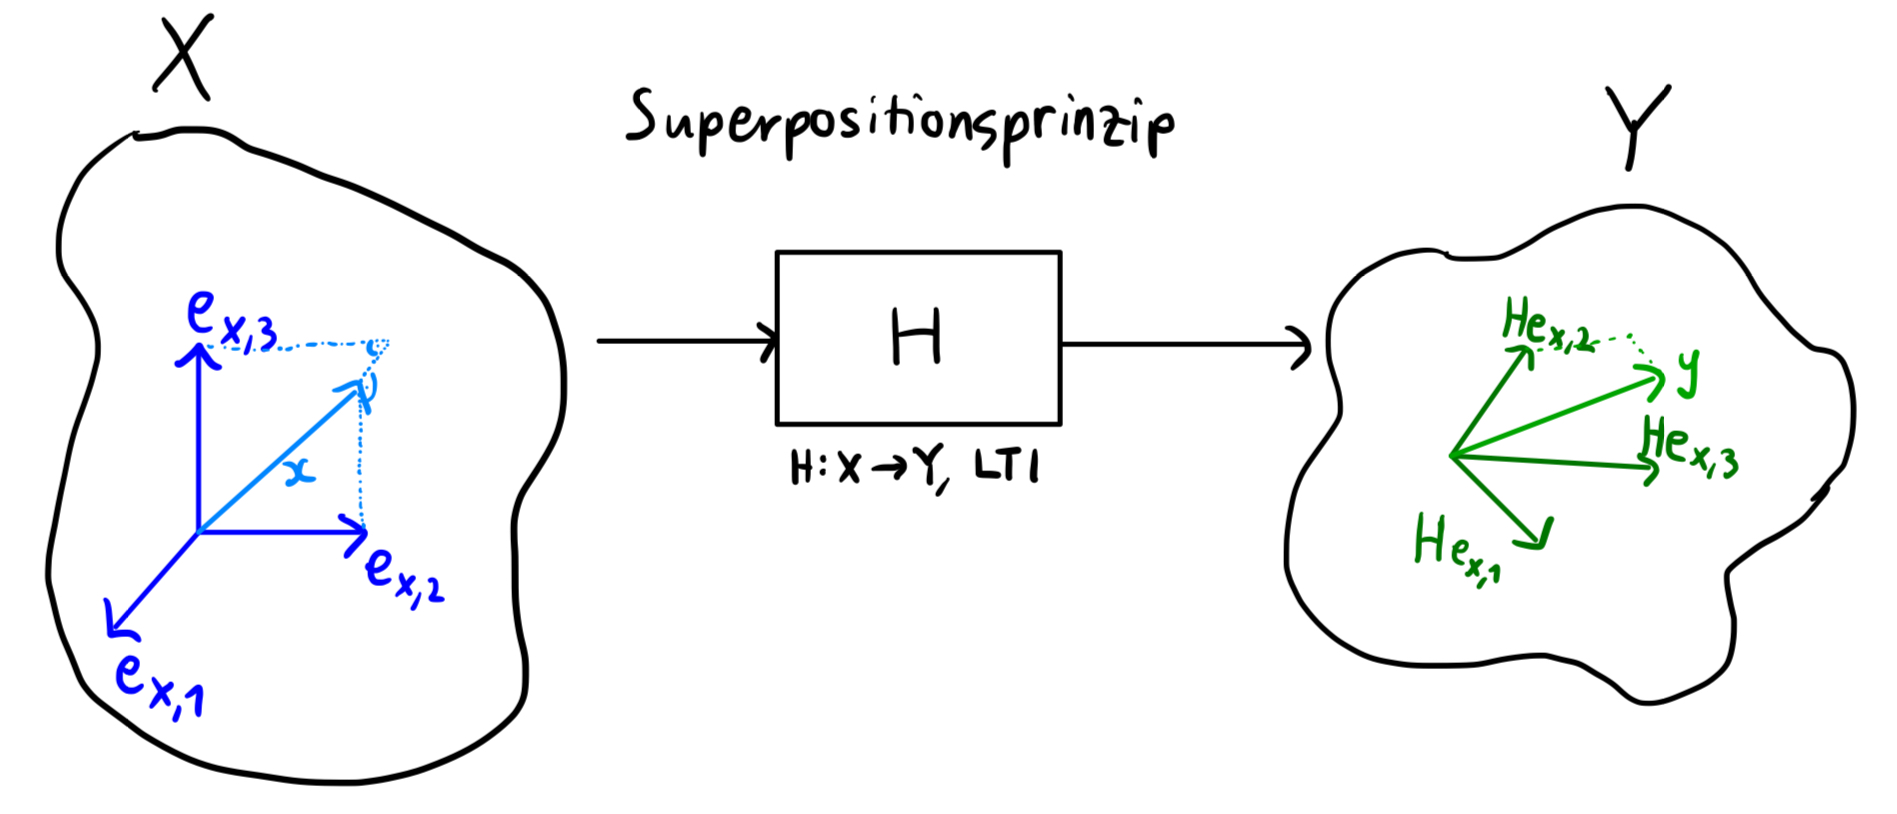
\includegraphics[width=0.8\linewidth]{figures/Superposition.jpeg}
    \end{center}
\end{frame}

\begin{frame}{Impulsantwort}
    \fcolorbox{darkblue}{lightblue}{\parbox{\dimexpr\linewidth-2\fboxsep-2\fboxrule\relax}{
    \textbf{\begin{center}
    LTI-Systeme sind vollständig durch ihre Impulsantwort $h := (H \delta)(t)$ definiert.
\end{center}} 
}}%

\vspace*{1cm}
Wir können dem System einen $\delta-$Impuls als Input geben und den Output betrachten und dieser Output charakterisiert das LTI-System vollständig.
\end{frame}

\begin{frame}{Herleitung}
    
\end{frame}

\begin{frame}{Herleitung}
    
\end{frame}

\begin{frame}{Herleitung}
    
\end{frame}

\begin{frame}{Impulsantwort von LTI-Systemen}
    \fcolorbox{darkblue}{lightblue}{\parbox{\dimexpr\linewidth-2\fboxsep-2\fboxrule\relax}{
    \begin{center}
    Ein LTI-System antwortet auf ein Eingangssignal $x(t)$ mit dem Ausgangssignal
    $$y(t) = \int_{-\infty}^\infty x(\tau)h(t-\tau)\text{d}\tau := x \ast h$$
    wobei $h(t) = (H\delta)(t)$ die \textbf{Impulsantwort} des Systems ist.
\end{center}
}}%
\end{frame}

\begin{frame}{Aufgabe 42.a)}
    
\end{frame}

\begin{frame}{Existenz des Faltungsintegrals}
    \begin{itemize}
        \item Das Faltungsintegral zweier Signale $x_1(t)$ und $x_2(t)$ $$(x_1 \ast x_2)(t) = \int_{-\infty}^{\infty} x_1(\tau)x_2(t-\tau) \text{d}\tau$$ kann divergieren.
        \item[] 
        \item Die \textbf{Young'sche Ungleichung} stellt sicher, dass eine Faltung zweier Signale existiert.
    \end{itemize}
\end{frame}

\begin{frame}{Repetition: $L^p$}
    \begin{itemize}
        \item $L^p := \left\{ x:\mathbb{R} \to \mathbb{C} \left| \displaystyle\int_{-\infty}^{\infty} |x(t)|^p \text{d}t < \infty \right. \right\}$
        \item[] 
        \item \textbf{p-Norm}: $||x||_p := \left(\displaystyle\int_{-\infty}^{\infty} |x(t)|^p \text{d}t\right)^{1/p}$
        \item[] 
        \item \textbf{Spezialfall}: $||x||_{\infty} := \inf\{C \geq 0: |x(t)| \leq C, \text{ für alle } t\in \mathbb{R}\}$
    \end{itemize}
\end{frame}

\begin{frame}{Young'sche Ungleichung: Theorem}
    \begin{itemize} 
        \item Seien $x$ und $h$ (messbare) Funktionen, sodass $||x||_p, \; ||h||_q < \infty$ für $p,q$ mit $1 \leq p,q \leq \infty$. Man setze:
        \item[] 
        $$\frac{1}{p} + \frac{1}{q} = 1 + \frac{1}{r}$$
        \item[] 
        \item[] Dann gilt: $||x \ast h||_r \leq ||x||_p||h||_q$.
    \end{itemize}
\end{frame}

\begin{frame}{Young'sche Ungleichung: Spezialfälle}
    \begin{itemize}
        \item $x_1 \in L^p, \; 1 \leq p \leq \infty, \; x_2 \in L^1 \implies ||x_1 \ast x_2 ||_p \leq ||x_1||_p ||x_2||_1$ und damit $x_1 \ast x_2 \in L^p$
        \item[] 
        \item $x_1 \in L^2, \; x_2 \in L^2 \implies |(x_1 \ast x_2 )(t)| \leq ||x_1||_2 ||x_2||_2, \; t \in \mathbb{R}$ \\und damit $x_1 \ast x_2 \in L^\infty$
    \end{itemize}
\end{frame}

\begin{frame}{Eigenschaften der Faltung}
    \begin{enumerate}
    \item \textbf{kommutativ}: $x_1 \ast x_2 = x_2 \ast x_1$
    \item[] 
    \item \textbf{assoziativ}: $x_1 \ast (x_2 \ast x_3) = (x_1 \ast x_2) \ast x_3$
    \item[] 
    \item \textbf{distributiv}: $x_1 \ast (x_2 + x_3) = x_1 \ast x_2 + x_1 \ast x_3$
    \item[] 
    \item \textbf{linear in beiden Argumenten}: $x_1 \ast (\alpha x_2 + \beta x_3) = \alpha (x_1 \ast x_2) + \beta (x_1 \ast x_3)$
\end{enumerate}
\end{frame}

\begin{frame}{Analytische Berechnung der Faltung: Aufgabe 41}
    
\end{frame}

\begin{frame}{Graphische Faltung: Kochrezept}
    \fcolorbox{darkblue}{lightblue}{%
\parbox{\dimexpr\linewidth-2\fboxsep-2\fboxrule\relax}{\begin{itemize}
    \item[] \textbf{Ziel}: Wir wollen $y(t) = \displaystyle\int_{-\infty}^{\infty} x(t-\tau)h(\tau) \text{d}\tau$ berechnen.
    \item[1)] $x(\tau)$ spiegeln um $\tau = 0$, um $x(-\tau)$ zu erhalten.
    \item[2)] Das gespiegelte $x(\tau)$ um $t$ verschieben.
    \item[] \vspace*{-0.5cm}\begin{multicols}{2}
        \begin{itemize}
        \item nach rechts für $t>0$
        \item[] $\implies x(t -\tau) = x(-(\tau-t))$
        \item nach links für $t<0$
    \end{itemize}
    \end{multicols}
    \item[3)] \vspace*{-0.5cm}Das gespiegelte \& verschobene $x(\tau)$ mit $h(\tau)$ multiplizieren. $\implies x(t-\tau)h(\tau)$
    \item[4)] Integrieren \& den Wert von $y(t)$ bei $t$ eintragen.
    \item[5)] Zurück zu 2) mit neuem $t$.
\end{itemize}
}}%
\end{frame}

\begin{frame}{Graphische Faltung: Hinweise}
    \textbf{Hinweise}: Vergesst nicht, dass die Faltung kommutativ ist, d.h.
    $$\int_{-\infty}^\infty x(t-\tau) h(\tau) \text{d}\tau = \int_{-\infty}^\infty x(\tau) h(t-\tau) \text{d}\tau$$
    Spiegelt und verschiebt das einfachere Signal und fixiert das kompliziertere!
\end{frame}

\begin{frame}{Aufgabe 39.a)}
    
\end{frame}

\begin{frame}{Eigenschaften der Impulsantwort}
    \begin{itemize}
        \item Kausalität
        \item[] 
        \item Gedächtnis
        \item[] 
        \item BIBO-Stabilität
    \end{itemize}
\end{frame}

\begin{frame}{Repetition: Kausalität}
    \begin{itemize}
        \item \textbf{Definition}: Ein System $H:X \to Y$ ist \textbf{kausal}, wenn für alle $x_1, x_2 \in X$ und jedes $T\in \mathbb{R}$ gilt
        \item[] 
        \item[] $x_1(t) = x_2(t), \hspace{10pt} \text{für alle } t \leq T $
        \item[] \vspace{0.25cm}$\implies (Hx_1)(t) = (Hx_2)(t), \hspace{10pt} \text{für alle } t \leq T$
    \end{itemize}
\end{frame}

\begin{frame}{Repetition: Kausalität}
    \begin{itemize}
        \item[] \begin{center}
        \includegraphics[width=0.8\linewidth]{figures/Kausalität.png}
        \end{center}
        \item \textbf{Intuition}: Das Ausgangssignal zu dem Zeitpunkt $T$ ist nur von dem momentanen oder vergangenen Zeitpunkten abhängig.
        \item[] 
        \item Echtzeitrealisierungen sind immer kausal.
    \end{itemize}
\end{frame}

\begin{frame}{Repetition: Gedächtnis}
    \begin{itemize}
        \item \textbf{Definition}: Ein System $H:X \to Y$ ist \textbf{gedächtnislos}, wenn für alle $x\in X$ und alle Zeitpunkte $t_0 \in \mathbb{R}$ das Ausgangssignal $(Hx)(t)$ zum Zeitpunkt $t_0$ nur von $x(t_0)$ abhängt.
        \item[] 
        \item Sonst heisst das System \textbf{gedächtnisbehaftet}.
        \item[] 
        \item Gedächtnislosigkeit $\implies$ Kausalität (aber nicht umgekehrt)
    \end{itemize}
\end{frame}

\begin{frame}{Repetition: BIBO-Stabilität}
    \begin{itemize}
        \item \textbf{Definition}: Ein System $H:X\to Y$ ist \textbf{BIBO-stabil}, wenn: 
        \item[] 
        \item[] für alle $x\in X$ mit $|x(t)| \leq B_x < \infty$, für alle $t$, existiert ein $B_y \in \mathbb{R}$ mit $B_y < \infty$, sodass 
        \item[] \vspace{0.25cm} $|y(t)| \leq B_y$, für alle $t$, wobei $y=Hx$.
    \end{itemize}
\end{frame}

\begin{frame}{Zusammenfassung: Eigenschaften der Impulsantwort}
    \fcolorbox{darkblue}{lightblue}{%
\parbox{\dimexpr\linewidth-2\fboxsep-2\fboxrule\relax}{
%\vspace*{-0.5cm}
\begin{itemize}
    \item[] \textbf{Kausalität}
    \item[] Das LTI-System ist kausal 
            $\Leftrightarrow h(t) = 0 \text{ für } t < 0.$
    \item[] 
    \item[] \textbf{Gedächtnislosigkeit}
    \item[] Das LTI-System $H$ ist gedächtnislos $\Leftrightarrow$
        $$y(t) = (Hx)(t) = \alpha x(t), \hspace{10pt} \alpha \in \mathbb{C} \Leftrightarrow h(t) = \alpha \delta(t) $$
    \item[] 
    \item[] \textbf{BIBO-Stabilität}
    \item[] Wenn $h \in L^1$, dann ist das LTI-System BIBO-stabil.
\end{itemize}
}}%
\end{frame}

\begin{frame}{Aufgaben}
    \begin{itemize}
        \item \textbf{Aufgabe 45}
        \item[]
        \item \textbf{Prüfungsaufgabe: Frühjahr 2024, Aufgabe 1}
    \end{itemize}
\end{frame}

\end{document}
